\documentclass[11pt, a4paper, DIV=12]{scrartcl}
\usepackage{amsmath}
\usepackage{amsfonts}
\usepackage{amssymb}
\usepackage{graphicx}
\graphicspath{{figs/}}
\usepackage{mathtools}
\usepackage{physics}
\usepackage{xcolor}
\usepackage{braket} % easy braket notation
\usepackage{enumitem}
\usepackage{booktabs}
\usepackage{here}
\usepackage{hyperref}
\usepackage{subcaption}
\usepackage[separate-uncertainty=true]{siunitx}

\usepackage[backend=biber, sorting=none]{biblatex}
\bibliography{refs.bib}

\author{Chenhuan Wang and Harilal Bhattarai}
\date{\today}
\title{Lab Report\\S261: Optical Astronomy and Gravitational Lensing}
\begin{document}
\maketitle

\begin{abstract}
	This is abstract.
\end{abstract}

\section{Introduction}

\section{Theory}
The partial decay width of $Z^0$ decay into fermion $f$ is
\begin{equation}
	\Gamma_f = \frac{ \sqrt{2} N_c^f}{12\pi} G_F M_Z^3 \left( (g_V^f)^2 + (g_A^f)^2  \right)
	\label{math:Gammaf}
\end{equation}
with
\begin{align*}
	g_V^f &= I_3^f - 2 Q_f \sin^2 \theta_W \\
	g_A^f &= I_3^f 
\end{align*}
One needs to be aware that $\Gamma_f$ contains contribution from both chiralities, and $I_3$ here refers to only the weak isospin of left-handed fermions (by definition right handed fermions have no weak isospin).

Partial cross section of $Z^0 \rightarrow f\bar{f}$ is given by~\cite{manual}
\begin{equation}
	\sigma_f(s) = \frac{12 \pi}{M_Z^2} \frac{s \Gamma_e \Gamma_f}{ (s-M_Z^2)^2 + (s^2 \Gamma^2_Z / M_Z^2)}
\end{equation}

In $ee \rightarrow ee$ scattering, two relevant channels have different angular dependences. For $s$-channel,
\begin{equation}
	\dv{\sigma}{\Omega}_s \sim (1 + \cos^2 \Theta)
	\label{math:diffCrossS}
\end{equation}
For $t$-channel,
\begin{equation}
	\dv{\sigma}{\Omega}_t \sim (1-\cos^2 \Theta)^{-2}
	\label{math:diffCrossT}
\end{equation}

\section{Preparatory Tasks}
\textbf{ P.3.1 Calculation of the deflection potential, $\psi(\theta) $ and the scaled deflection angle of an SIS lens.}\\
 
 \noindent
 From equation \ref{psiTheta} the deflection potential, which gives the information about the mass distribution of the lens, is define as,
 \begin{equation}
 \psi(\theta)=\frac{1}{\pi}\int d^2\theta'\kappa(\theta')\ln |\theta-\theta'| 
 \end{equation}
 In the case of axial symmetry of SIS lens equation \ref{psiTheta} simplifies to (given on the question)
 \begin{equation}
 \psi(\theta)=2\int_{0}^{\theta}d\theta' \theta'\kappa(\theta') \ln \bigg(\frac{\theta}{\theta'}\bigg)
 \label{Equ:psiSIS}
 \end{equation}

 By substituting the values of $ \Sigma(D_{d}\theta) $, where $ D_{d}\theta=\xi $ from equation \ref{equ:Sigma(xi)} and  $ \Sigma_{cr} $ from equation \ref{SumCr} on equation \ref{Equ:KTheta}, then by plugging the new expression of  $ \kappa(\theta) $ equation \ref{Equ:psiSIS} becomes
 
 
 \begin{align*}
	 \psi(\theta)&=\frac{4\pi}{c^2}\frac{D_{ds}}{D_{s}}\sigma^2_{v}\int_{0}^{\theta}d\theta' ln \bigg(\frac{\theta}{\theta'}\bigg) \\
					 &=\frac{4\pi}{c^2}\frac{D_{ds}}{D_{s}}\sigma^2_{v} \left[\theta' \ln(\frac{\theta}{\theta'})+\theta'\right] \\
					 &=\theta_{E}(\theta \ln \theta - \theta \ln \theta + \theta )
 \end{align*}
 Therefore, 
 \begin{equation}
 \psi(\theta)=\theta_{E}\theta 
 \label{Equ:psiFinal}
 \end{equation}
 From equation \ref{Equ:AlphaTheta} scaled deflection angle is defined as
 \begin{equation}
 \alpha(\theta)=\nabla\psi(\theta)
 \label{Equ:AlphaTheta2}
 \end{equation}
 From equations: \ref{Equ:psiFinal} and \ref{Equ:AlphaTheta2},
 \begin{equation}
 \alpha(\theta)=\nabla \theta_{E}\theta = \theta_{E}\hat{\theta}
 \label{Equ:AlphaThetaFinal}
 \end{equation}
 \\
 
 \textbf{P.3.2: Solving the lens equation and finding the separation between images}\\
 
 The lens equation is given by,
 \begin{equation}
 \beta=\theta-\alpha(\theta)
 \end{equation}
 By using the expression for scaled deflection angle for SIS from \ref{Equ:AlphaThetaFinal}
 \begin{equation}
 \beta=\theta-\theta_{E}\hat{\theta}
 \end{equation}
 or, 
 \begin{equation*}
 \alpha(\theta)=\beta+\theta_{E}\hat{\theta}
 \end{equation*}
 for $ \hat{\theta}>0 $,
 \begin{equation*}
 \theta_{A}=\beta + \theta_{E}
 \label{Equ:ThetaA}
 \end{equation*}
 for $ \hat{\theta}<0 $,
 \begin{equation*}
 \theta_{B}=\beta -\theta_{E}
 \label{Equ:ThetaB}
 \end{equation*}
 Thus, the separation of these  images is given by,
 \begin{equation}
 \Delta\theta= \theta_{A}- \theta_{B} = 2\theta_{E}
 \label{math:imSep}
 \end{equation}
 \\
 
 \textbf{P.3.3: Magnification ratio of the two images of SIS lens.}\\
 
 The magnification of a gravitational lens is given by,
 \begin{equation}
 \mu=(det \text{A})^{-1}
 \end{equation}\\
 
 
 
 
 
 \textbf{P.3.4: Time delay derivation for SIS lens as a function of $ \theta_{A}$ and $ \theta_{B}$.}\\
 
 The time delay is given by\cite{manual}
 \begin{equation}
 \text{c}\Delta\text{t}(\beta)=(1+ \text{z}_{d})\frac{\text D_{d}D_{s}}{D_{ds}}[\tau(\theta_{A};\beta) - \tau(\theta_{B}; \beta)]
 \label{Equ:timeDelay}
 \end{equation}
 
 Also, from \ref{Equ:Format} the Format's potential is defined as,
 \begin{equation}
 \tau(\theta; \beta)=\frac{1}{2}(\beta -\alpha)^2 -\psi(\theta)
 \end{equation}
 So,
 
 \begin{equation}
 \tau(\theta_{A}; \beta)=\frac{1}{2}(\beta -\theta_{A})^2 -\psi(\theta_{A})
 \end{equation}
 By plugging the values of $\beta$ and $\psi(\theta_{A})$,
 \begin{equation}
 =\frac{1}{2}(\theta_{A}-\theta_{E} -\theta_{A})^2 -\theta_{E}\theta_{A}
 \end{equation}
 Therefore,
 \begin{equation}
 \tau(\theta_{A}; \beta)=\frac{1}{2}\theta^2_{E} -\theta_{E}\theta_{A}
 \end{equation}
 
  Similarly,
  \begin{equation}
  \tau(\theta_{B}; \beta)=\frac{1}{2}(\beta -\theta_{B})^2 -\psi(\theta_{B})
  \end{equation}
  
   \begin{equation}
   =\frac{1}{2}(\theta_{B}+\theta_{E} -\theta_{B})^2 -\theta_{E}\theta_{B}
   \end{equation}
 
   \begin{equation}
  \tau(\theta_{B}; \beta) =\frac{1}{2}\theta^2_{E} - \theta_{E}\theta_{B}
   \end{equation}
  By substituting these values equation \ref{Equ:timeDelay} becomes, 
 \begin{equation}
 \text{c}\Delta\text{t}(\beta)=(1+ \text{z}_{d})\frac{\text D_{d}D_{s}}{D_{ds}}(\frac{1}{2}\theta^2_{E} -\theta_{E}\theta_{A} - \frac{1}{2}\theta^2_{E} + \theta_{E}\theta_{B})
 \end{equation}
  Therefore,
  
  \begin{equation}
  \Delta\text{t}(\beta)=\frac{(1+ \text{z}_{d})}{\text{c}}\frac{\text D_{d}D_{s}}{D_{ds}}\theta_{E}(\theta_{B}-\theta_{A})
  \end{equation}
  Thus, the time delay is proportional to the Einstein radius.\\
  
  
  
  \textbf{P.3.5: Minimum Dispersion Estimator}\\
  
  \noindent
  The minimum dispersion estimator is a simple, efficient and well tested method to estimate time delay from observed light curve\cite{manual}
  It helps to fine the difference between the curve at various delay times.
  Since it assume that light curves have the same shape but they are separated by time.\\
  
  
  \textbf{P3.6: The approximation of dispersion function near the minimum by a parabola.}\\
  
  The dispersion function near the minimum can be find by Taylor expanding of the functional function. i.e.
  
  \begin{equation}
  d^2(\lambda)=D^2(\lambda_{0}) +\frac{\text{d}D^2(\lambda_{0})}{\text{d}\lambda}(\lambda- \lambda_{0}) + \frac{\text{d}^2 D^2(\lambda_{0})}{\text{d}\lambda^2}(\lambda - \lambda_{0})^2 + 0
  \label{Equ:lambda}
  \end{equation}
  Where, $ \text{D}^2 $ is the dispersion function and $ \lambda $ is the time shift.
  Here high order terms are negligible compared to first and second order terms.\\
  
  The dispersion function is minimum at $ \lambda= \lambda_{0} $. Now the second term of equation \ref{Equ:lambda} goes to zero. i.e.
  
  \begin{equation}
  d^2(\lambda)=D^2(\lambda_{0}) + \frac{\text{d}^2 D^2(\lambda_{0})}{\text{d}\lambda^2}(\lambda - \lambda_{0})^2 
  \end{equation}
  it is parabolic in shape.

\section{Experimental procedure}
\subsection{Adjusting the gain of the Amplifier}
First, we adjusted the gain of both amplifiers  ($A_{1}$ and  $A_{2}$) during the set up of the experiment.We visualized the signal with the help of Oscilloscope. Following figure shows the amplified signal from the Amplifier1.



\begin{figure}[htbp]
	\centering
	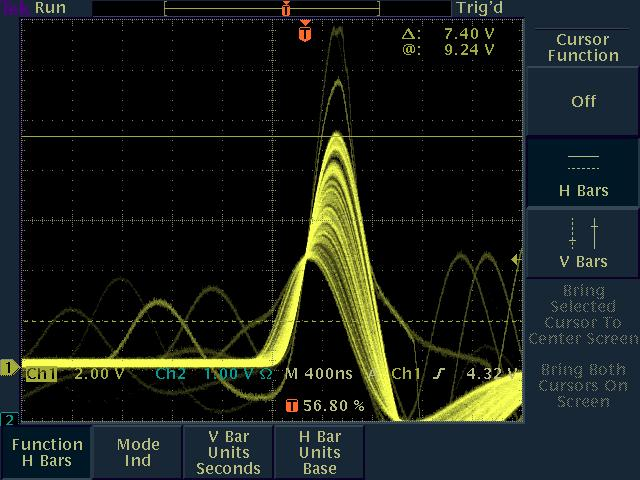
\includegraphics[width=0.8\linewidth]{./figs/amplified.jpg}
	\caption{Amplified Signal Output from the Detector.}%
	\label{fig:angAsymm}
\end{figure}

\subsection{Adjusting of the CFD}
CFD has a threshold-discriminator which help to filter out zero crossing that belongs to electronic noise and not to a true scintillation signal. So, we have adjusted this threshold of CFD to detect only true signals not the background noise signals. In that step, We connected the negative outputs of the both CFDs to the counters and measured the count rates with and without source installed.

\begin{figure}[htbp]
	\centering
	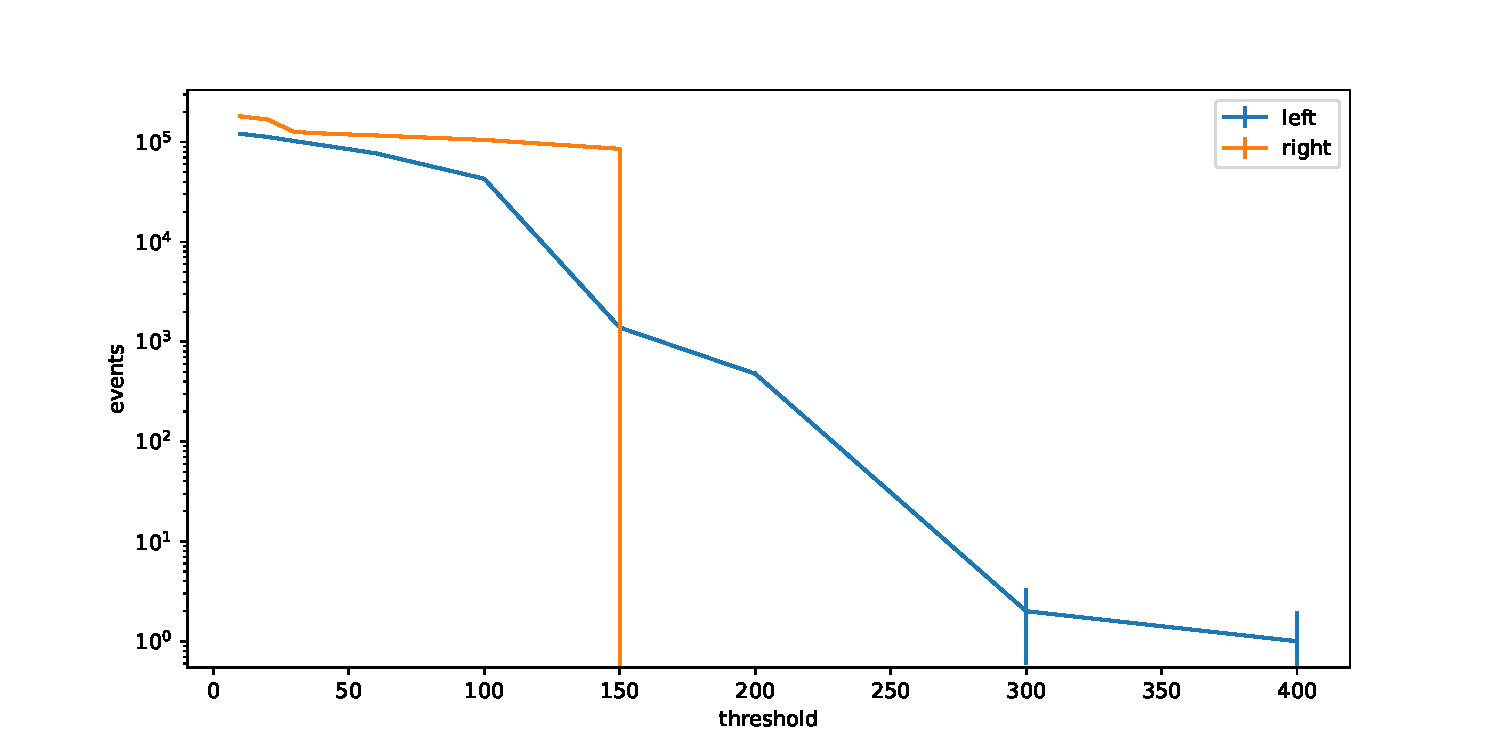
\includegraphics[width=0.8\linewidth]{./figs/cfd.pdf}
	\caption{CFD count rate with inserting source. Here threshold limit is [150-400] and in the end threshold to 30. }%
	\label{fig:angAsymm}
\end{figure}

\begin{figure}[htbp]
	\centering
	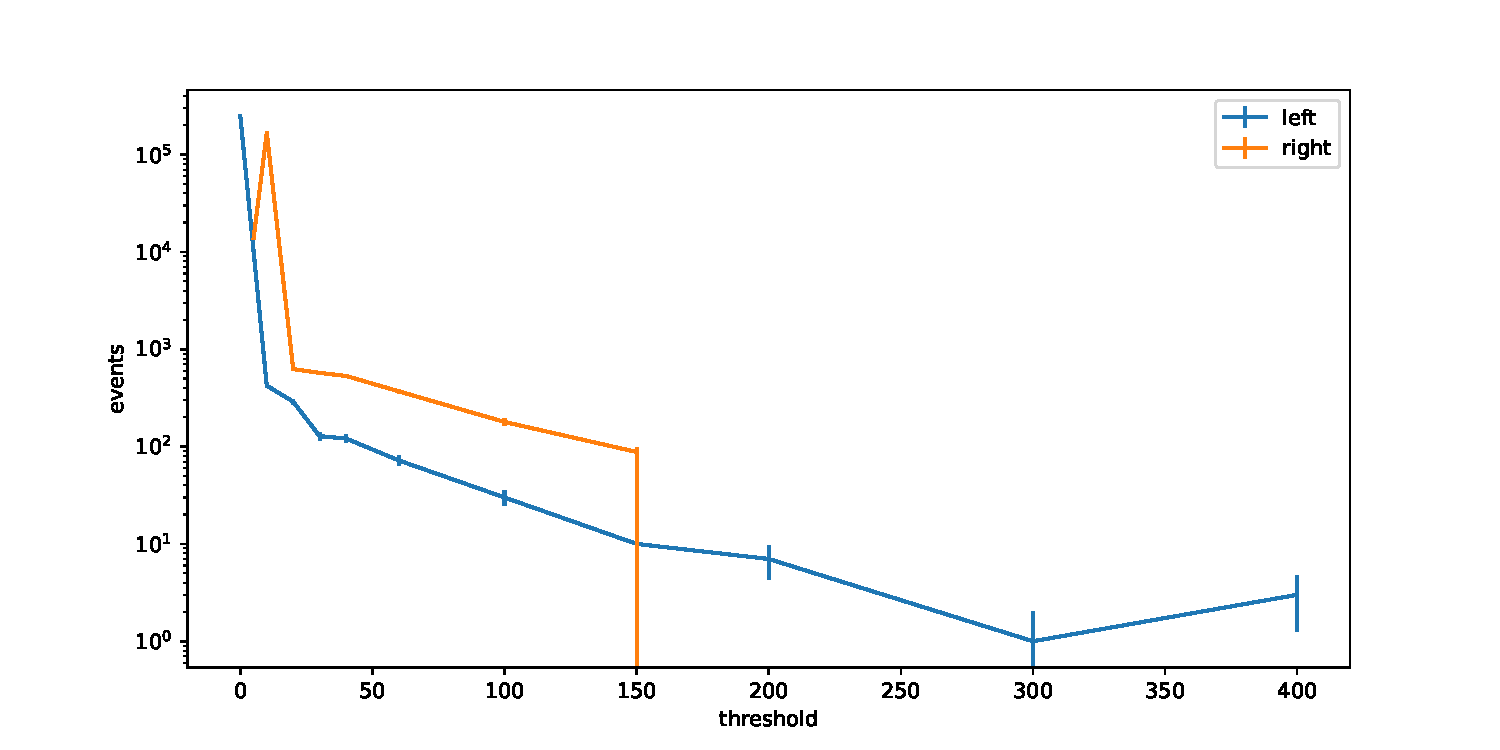
\includegraphics[width=0.8\linewidth]{./figs/cfd2.pdf}
	\caption{CFD count rate without inserting source. Here threshold limit is [150-400] and in the end threshold to 30.}%
	\label{fig:angAsymm}
\end{figure}

\subsection{Setting up the Fast Coincidence}
In this step, we visualized the coincidence of incoming signals from two CFDs with th help of oscilloscope and then determined the proper delay.For that, we connected the negative outputs of both CFDs to the oscilloscope and triggered on the first channel signals.Then, on the second channel, true coincidence appeared. Then, we inserted the fixed delay in between CFD1 and FC and a variable delay in between CFD2 and FC. After that, we picked the resolving time for FC as 25 ns.

\subsection{Setting up the Slow Coincidence}
Here, we connected the output from the fast coincidence unit to a gate and delay ($ D^{2}-G^{2} $) generator module. Also, the delay of both SCAs can be adjusted. Then, the output from ($ D^{2}-G^{2} $) inserted to the first channel and positive output from SCA1 and SCA2 on after another to th second channel of the oscilloscope. Afterward, we adjusted the delays in both SCAs and ($ D^{2}-G^{2} $). 

\subsection{Calibrating th Signal Channel Analyzer}
In this step, we performed the energy calibration and recorded the energy spectrum by using SCAs. For that, we set the SCA to the window mode. Later  we keep thee constant obtained window width for our measurement. Figure 7 and figure 8 shows the energy spectrum of $ ^{60}Co$-decay obtained by SCA1 and SCA2 respectively.
\begin{figure}[ht]
	\centering
	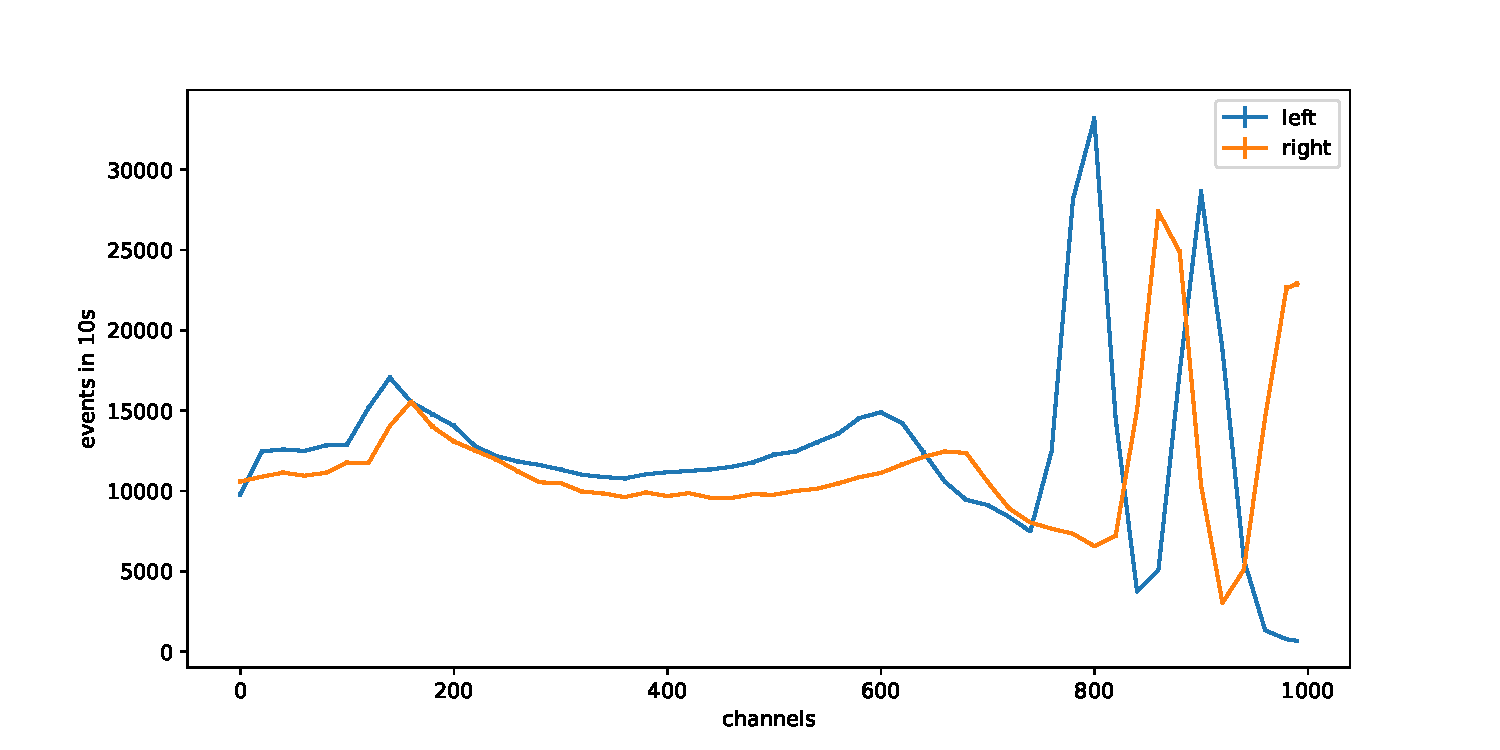
\includegraphics[width=0.8\linewidth]{./figs/sca.pdf}
	\caption{The energy spectra of SCA1. Here two peaks are in the range of [750-1000].}%
	\label{fig:angAsymm}
\end{figure}

\begin{figure}[ht]
	\centering
	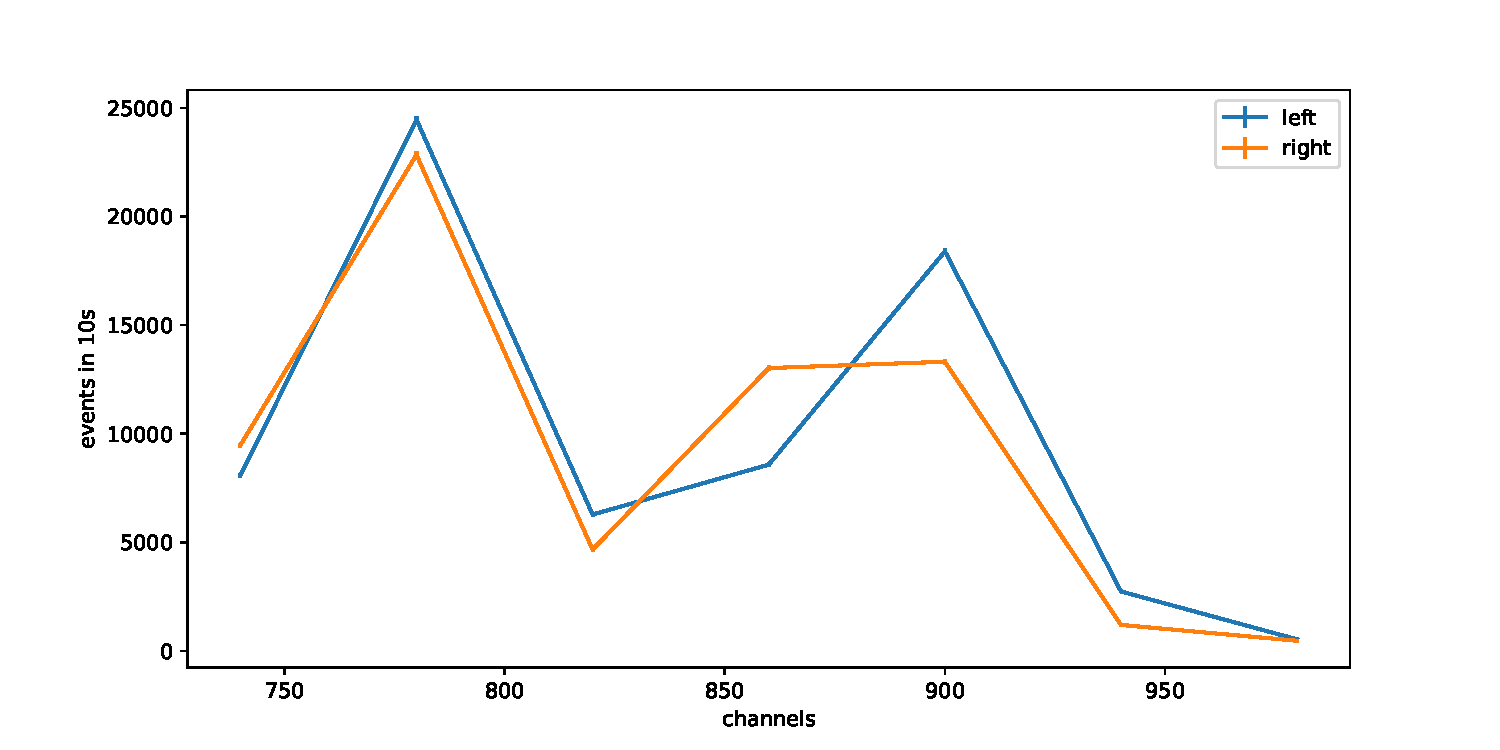
\includegraphics[width=0.8\linewidth]{./figs/sca2.pdf}
	\caption{The energy spectra of SCA2. Here two peaks are in the range of [750-950].}%
	\label{fig:angAsymm}
\end{figure}


\subsection{Main Measurement}
After adjusting all the involving apparatus in the experiment, we stated to perform th main measurement of the experiment. we used two detectors: on of them is fixed and another is movable. We inserted both detectors 5cm apart from the source. Then we measured the count rates for different angles between these two detectors.

\begin{figure}[ht]
	\centering
	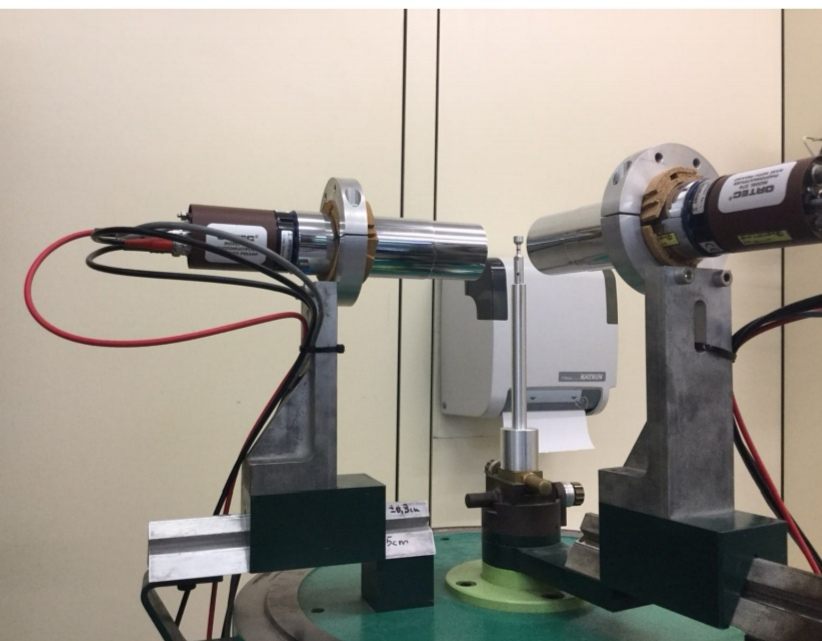
\includegraphics[width=0.8\linewidth]{./figs/detectors.jpg}
	\caption{Set up of two detectors where one is fixed and another one is movable to rotate at a fixed radial distance from the fixed detector.}%
	\label{fig:angAsymm}
\end{figure}



\clearpage
\section{Lensing analysis} 
\paragraph{Calculation with accepted value of $H_0$}
Since the redshifts of lens and source system are known, one can from image separation determine the velocity dispersion in SIS model. Angular distances should be computed also by equation.~\ref{math:Dangular2}. Here the cosmological parameters are taken from~\cite{planck}
\begin{equation*}
	\Omega_m = \num{0.3089 +- 0.0062}, \quad \Omega_\Lambda=\num{0.6911 +- 0.0062}
\end{equation*}
For simplicity, errors in these parameters are not propagated in further analysis (almost negligible). For this part, currently accepted value of $H_0$ is used.

Image separation can be used to compute Einstein radius. Results of \verb|galfit| are in pixels, so they need to be converted to angles first. As given in~\cite{alfa-manual}, the field of view of Cassegrain focus is $21'\times14'$, meaning one pixel corresponds to $0.4''$. Image separation can be expressed by Einstein radius with equation.~\ref{math:imSep}. The separation in pixels and in radians are then
\begin{align*}
	\Delta r &= \num{6.60 +- 0.079} \, \text{(pixels)} \\
	\Delta \theta &= (\num{1.281 +-0.015}) \cdot 10^{-5} = 2 \theta_E
\end{align*}
Here the error is properly propagated using
\begin{align*}
	\sigma_{\Delta r} ^2 &= \left( \pdv{\Delta r}{x_A}  \right)^2 \sigma_{x_A}^2 + \left( \pdv{\Delta r}{y_A}  \right)^2 \sigma_{y_A}^2 + \left( \pdv{\Delta r}{x_B}  \right)^2 \sigma_{x_B}^2 + \left( \pdv{\Delta r}{y_B}  \right)^2 \sigma_{y_B}^2 \\
								&= \frac{1}{(\Delta r)^2} \left[ (x_A - x_B)^2(\sigma_{x_A}^2 + \sigma_{x_B}^2) + (y_A - y_B)^2 (\sigma_{y_A}^2 + \sigma_{y_B}^2) \right]
\end{align*}

With equation.~\ref{Equ:ThetaE}, one finds
\begin{equation}
	\sigma_v = (\num{9.913 +- 0.597 })\cdot 10^{-4} c
\end{equation}
where the error is given by
\begin{equation*}
	\sigma_{\sigma_v} = \frac{\sigma_v}{2\theta_E} \sigma_{\theta_E}
\end{equation*}

According to equation.~\ref{math:projMass}, projected mass inside Einstein radius is computed to be
\begin{equation}
	M(\theta < \theta_E) = (\num{5.766 +- 0.139}) \cdot 10^{11} M_\odot
\end{equation}
This has similar magnitude as the estimated mass of milky way ($\sim \num{1e12} M_\odot$)~\cite{Grand_2019}. The error is propagated to be
\begin{equation*}
	\sigma_{M} = \frac{2M}{\theta_E} \sigma_{\theta_E}
\end{equation*}

\paragraph{Determination of $H_0$}

\section{Conclusion}\label{sec:conclusion}
In this experiment, we measured angular correlation between two photons emitted from ${}^{60}\text{Co}$. Then, the data gets fitted with the theoretical prediction function and  the angular correlation coefficients are calculated:  $ A_{22}= \num{0.0849 +- 0.0057} $ and $A_{44}=\num{-0.0002 +- 0.0063} $. The non-zero values of these two angular correlation coefficients provide strong evidence for an angular correlation between two gamma rays emitted in 420 cascade of $ ^{60}\text{Co} $. Via curve fitting, we can conclude that other types of cascade (020,121, 220, and 320) are basically $100\%$ excluded.

Further investigation reveals that measured values differ from prediction by $4\sigma$ due to unknown systematic errors in the setup. One of these systematic errors could very well be in electronics. Geometry of the setup could be measured and investigated more. As mentioned before, the resolving time can be lowered a bit. But it should not have huge impact on determination of angular correlation coefficients. 

\section{Acknowledgement}
We would heartly acknowledge the Bonn-Cologne Graduate School of Physics and Astronomy (BCGS) for the opportunity to perform the experiment. We would like to express our gratitude and appreciation for Dr. Christian Honisch for the tutoring, encouragement, and guidance throughout the experiment.



\clearpage
\printbibliography
\end{document}
